\documentclass[12pt,aspectratio=169]{beamer}
\usetheme{Madrid}
% CJK support
\usepackage{ctex}
\usepackage[utf8]{inputenc}
\usepackage[english]{babel}
\usepackage{amsmath}
\usepackage{amsfonts}
\usepackage{amssymb}
\usepackage{graphicx}
\usepackage{url}
\usepackage{hyperref}


%\bibliographystyle{apalike}
%\bibliography{Biblio}														% *.bib file with bibliography entries

% content definition

\author{Dali Cao, Kido Zhang}
\title{Tool Wear Prediction With Convolutional Neural Networks}

\subtitle{使用残差剩余卷积网络预测刀具磨损}

\logo{\includegraphics{picture/npu_logo_transparent.pdf}}

\institute[NWPU]{西北工业大学机电学院}

\date{\today}

\subject{}

\setbeamercovered{transparent}

\setbeamertemplate{navigation symbols}{}

\begin{document}
	% title page
	\maketitle
	
	\begin{frame}
		\frametitle{目录}
		% reduce work
		\setcounter{tocdepth}{1}
		\tableofcontents
	\end{frame}
	\section{概述}
	\subsection{刀具的磨损量检测}
	
	\begin{frame}
		\frametitle{刀具的磨损量检测}
		
		\begin{block}{概念}
			通过一系列的传感器技术得到信号,进而以此预测刀具的磨损量
		\end{block}
		
		\begin{block}{重要性}
			约有7-20\%的机器的宕机原因都是刀具的磨损,这也是生产力下降的一个非常重要的原因\cite{kegg1984one,kurada1997review}
		\end{block}
		
		\begin{block}{难题}
			刀具磨损量的检测仍然有很多基于Taylor\cite{marksberry2008comprehensive}刀具寿命等式的模型以供参考,然而其并没有考虑加工中的不稳定性。
		\end{block}
		
	\end{frame}
	
	
	\subsection{当今预测的工具}
	
	\begin{frame}{当今手段}
		如今大量的人工智能算法都广泛的处理来自测力计,加速度计,声发射和电流功率传感器的数据\cite{cho1999state}
		
		步骤有:
		
		\begin{enumerate}
			\item 进行加工实验
			\item 通过传感器得到信号
			\item 信号的预处理(放大或者滤波)
			\item 特征提取
			\item 使用算法生成模型并且训练数据
			\item 预测结果
		\end{enumerate}
		
		
%		\par 常见的算法有
%		
%		\begin{itemize}
%			\item 神经网络
%			\item 神经模糊模型
%			\item 混沌算法
%			\item 贝叶斯网络
%		\end{itemize}
	\end{frame}
	
	\subsection{卷积神经网络}
	
	\begin{frame}
		\frametitle{卷积神经网络}
		\begin{block}{为什么使用卷积神经网络?}
			\begin{itemize}
				\item 因为输入数据具有局部相关性
				\item 输入数据在局部特征也具有平移不变性,也就是说在不同位置都具有共性的局部特征,这样在多层堆叠下,底层局部特征可以抽取成高层全局特征。
				\item 权值共享则可以大大降低网络的训练难度
				
			\end{itemize}
			
		\end{block}
		\begin{block}{为什么需要使用残差结构来构造神经网络}
			\begin{itemize}
				\item 能有效的解决梯度消失的问题
				\item 能够搭建更深的神经网络,使得神经网络的表达能力更强
			\end{itemize}
		\end{block}
	\end{frame}
	
	\section{实验方法}
	\subsection{信号获得与处理}
	\begin{frame}{信号来源和其预处理}
		\begin{block}{数据来源}
			所有的加工数据来自于PHM学会2010关于刀具磨损量的数据\cite{phm2010}
		\end{block}
		
		\begin{block}{数据预处理 - 小波变换}
			对信号进行等数量的时间步长均匀采样,并对每个维度的信号进行小波变换,得到两层高频和一层低频信号,进而拼接作为神经网络的输入
		\end{block}
		
		
		
		
	\end{frame}
	
	\subsection{神经网络的搭建}
	
	\begin{frame}{神经网络模型}
		我们使用了残差剩余卷积神经网络来处理模型,其使用Keras(后端是基于GPU的Tensorflow)框架编写。
		
		\begin{itemize}
			\item 使用了较深的网络(10-30)来表达这个过程
			\item 使用平均方差来作为误差函数训练
			\item 使用Adam优化器来训练整个模型
		\end{itemize}
		
	\end{frame}
	
	\section{深度学习实验以及结果}
	
	\subsection{机器的设置和处理}
	
	\begin{frame}{机器的设置和处理}
		\begin{block}{数据预处理}
			整个实验运行在工作站上,其使用的是一块Quadro M2000显卡。整个实验数据首先经过小波变换后,手动打乱整个数据集,然后按照训练集数据集0.8:0.2划分。
		\end{block}
		
		\begin{block}{网络的选择}
			使用函数式模型搭建整个残差剩余网络,以三个不同的波形作为输入,输出是三齿的磨损量。残差剩余网络的网络深度按照5,10,20,30取值。以亚当优化器作为模型的优化器,以平均平方误差作为损失函数,以保证整个问题是一个凸函数的问题。
		\end{block}
		
		\begin{block}{过程监控}
			使用TensorBoard监控整个训练过程,得到每个训练周期内的损失值。
		\end{block}
		
		
	\end{frame}
	
	\subsection{实验过程}
	\begin{frame}{实验过程}
		采用Adam算法,测试不同深度的残差剩余网络,并且在其中选择loss最低的结果作为最终的模型。
		
		( 开Tensorboard手动演示。。。 )
		
	\end{frame}
	
	
	\subsection{实验结果}
	\begin{frame}{综述}
		根据我们的预测结果和实验值结果,在残差神经网络深度为15层的时候,其在训练和验证集的效果最佳。同时可以得到如图所示的概率分布曲线。
		
		算法在以Quadro M2000的CUDNN计算环境下,预测945个小切削过程的刀具磨损计算时间在0.2-0.3秒内。
	\end{frame}
	
	
	
	\begin{frame}{实验结果}
		\centering
		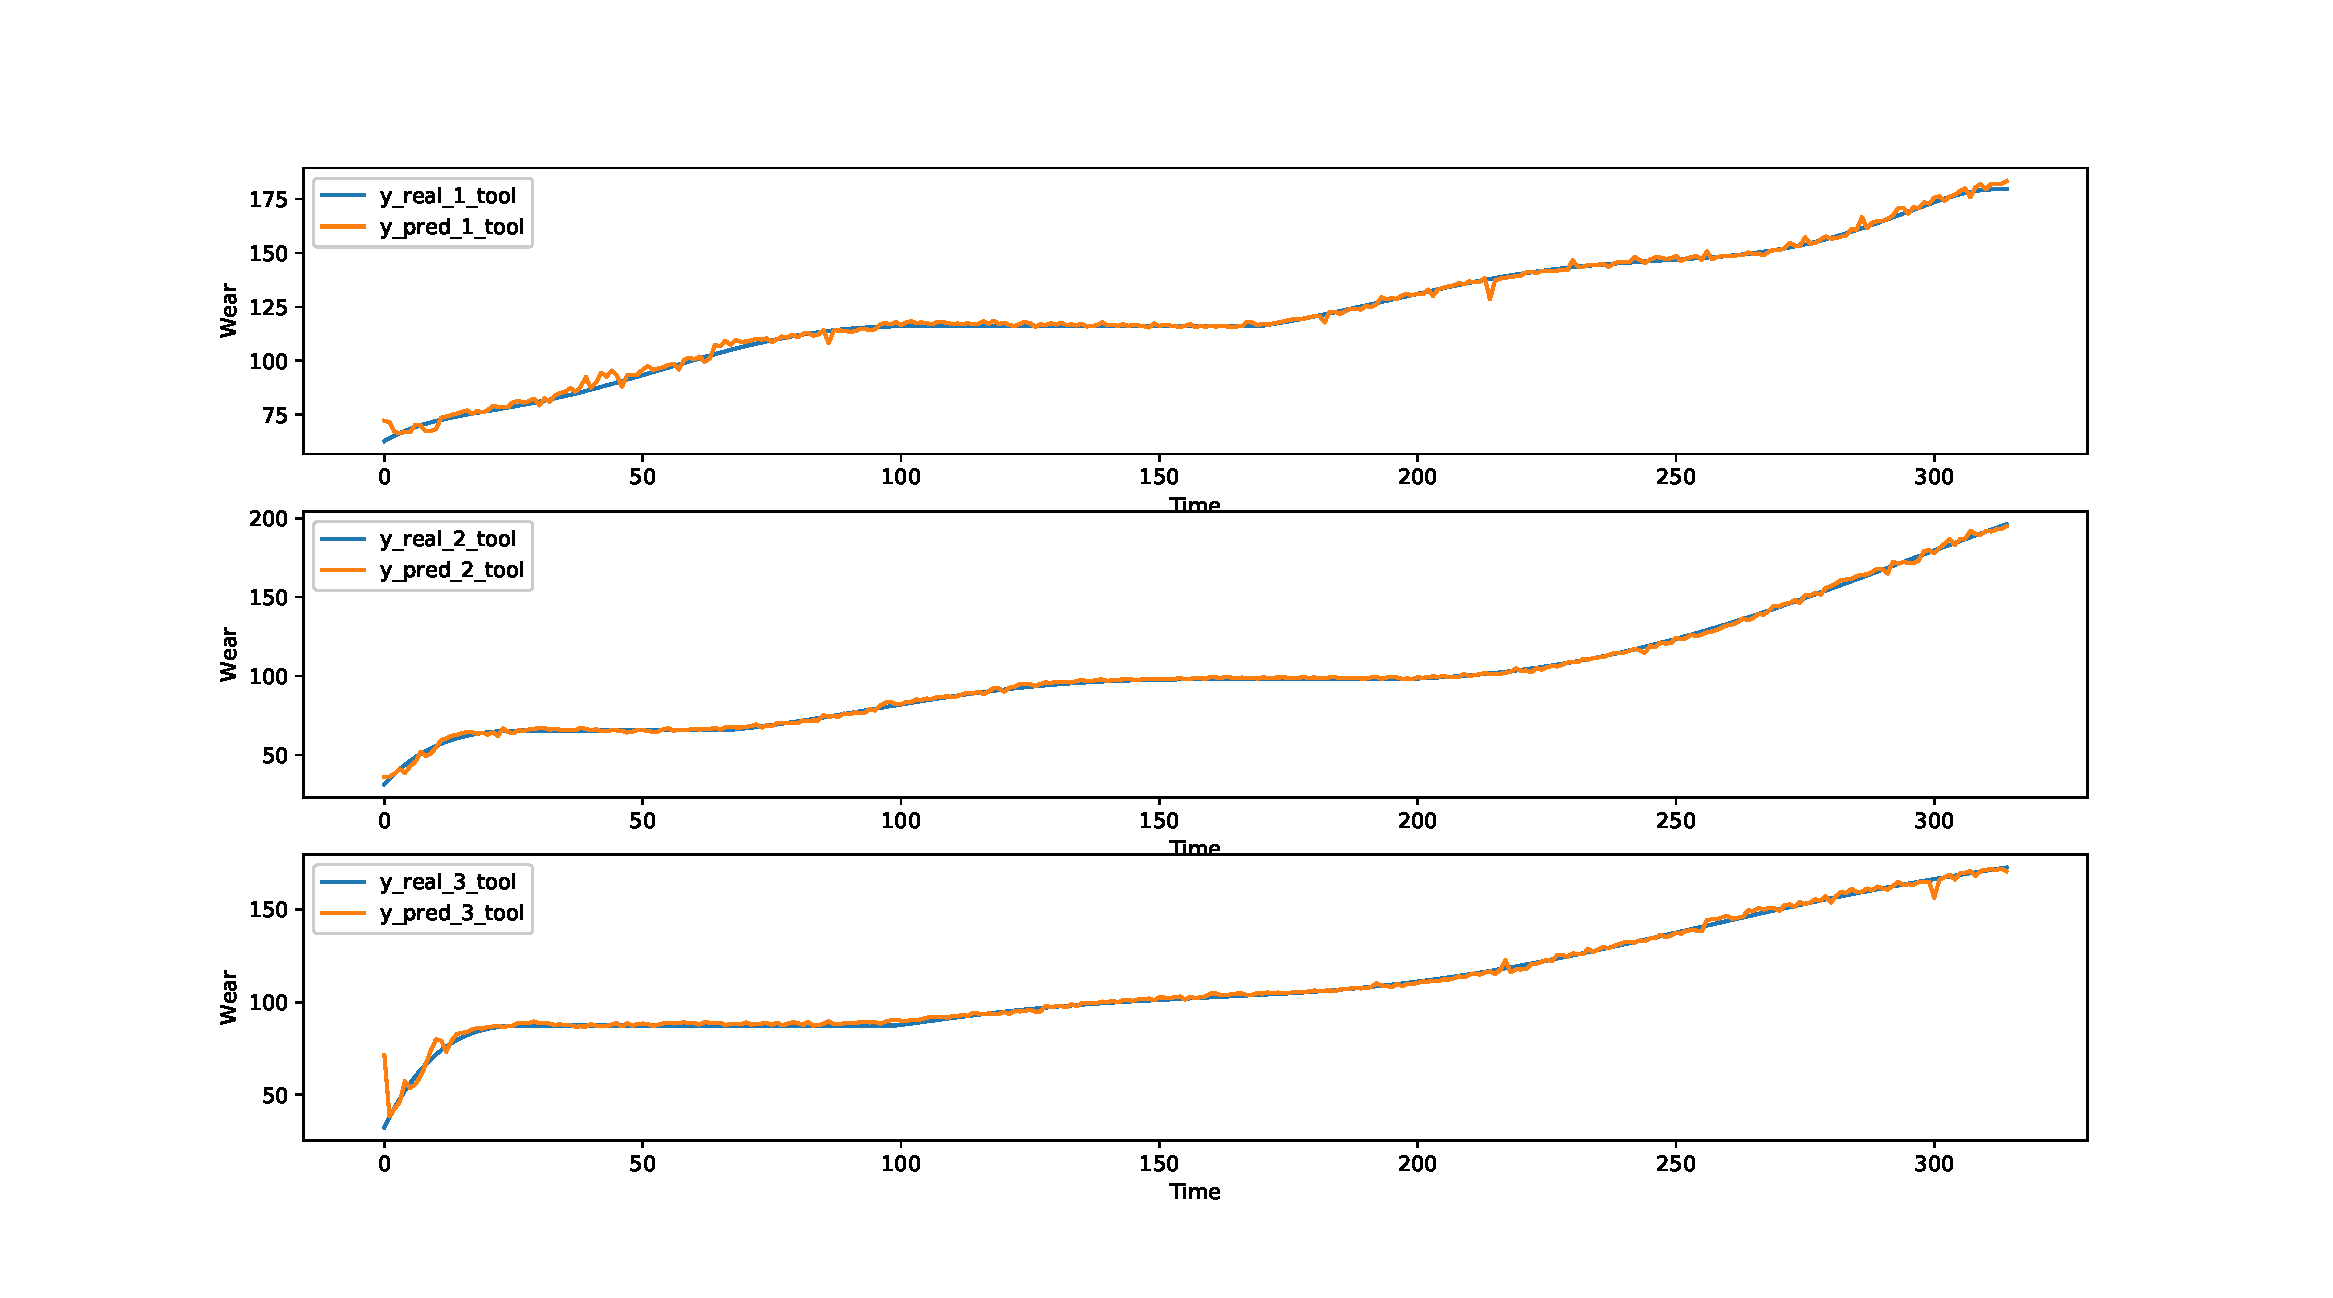
\includegraphics[height=0.9\textheight]{picture/x_tool}

	\end{frame}
	
	\begin{frame}{实验结果}
		\centering
		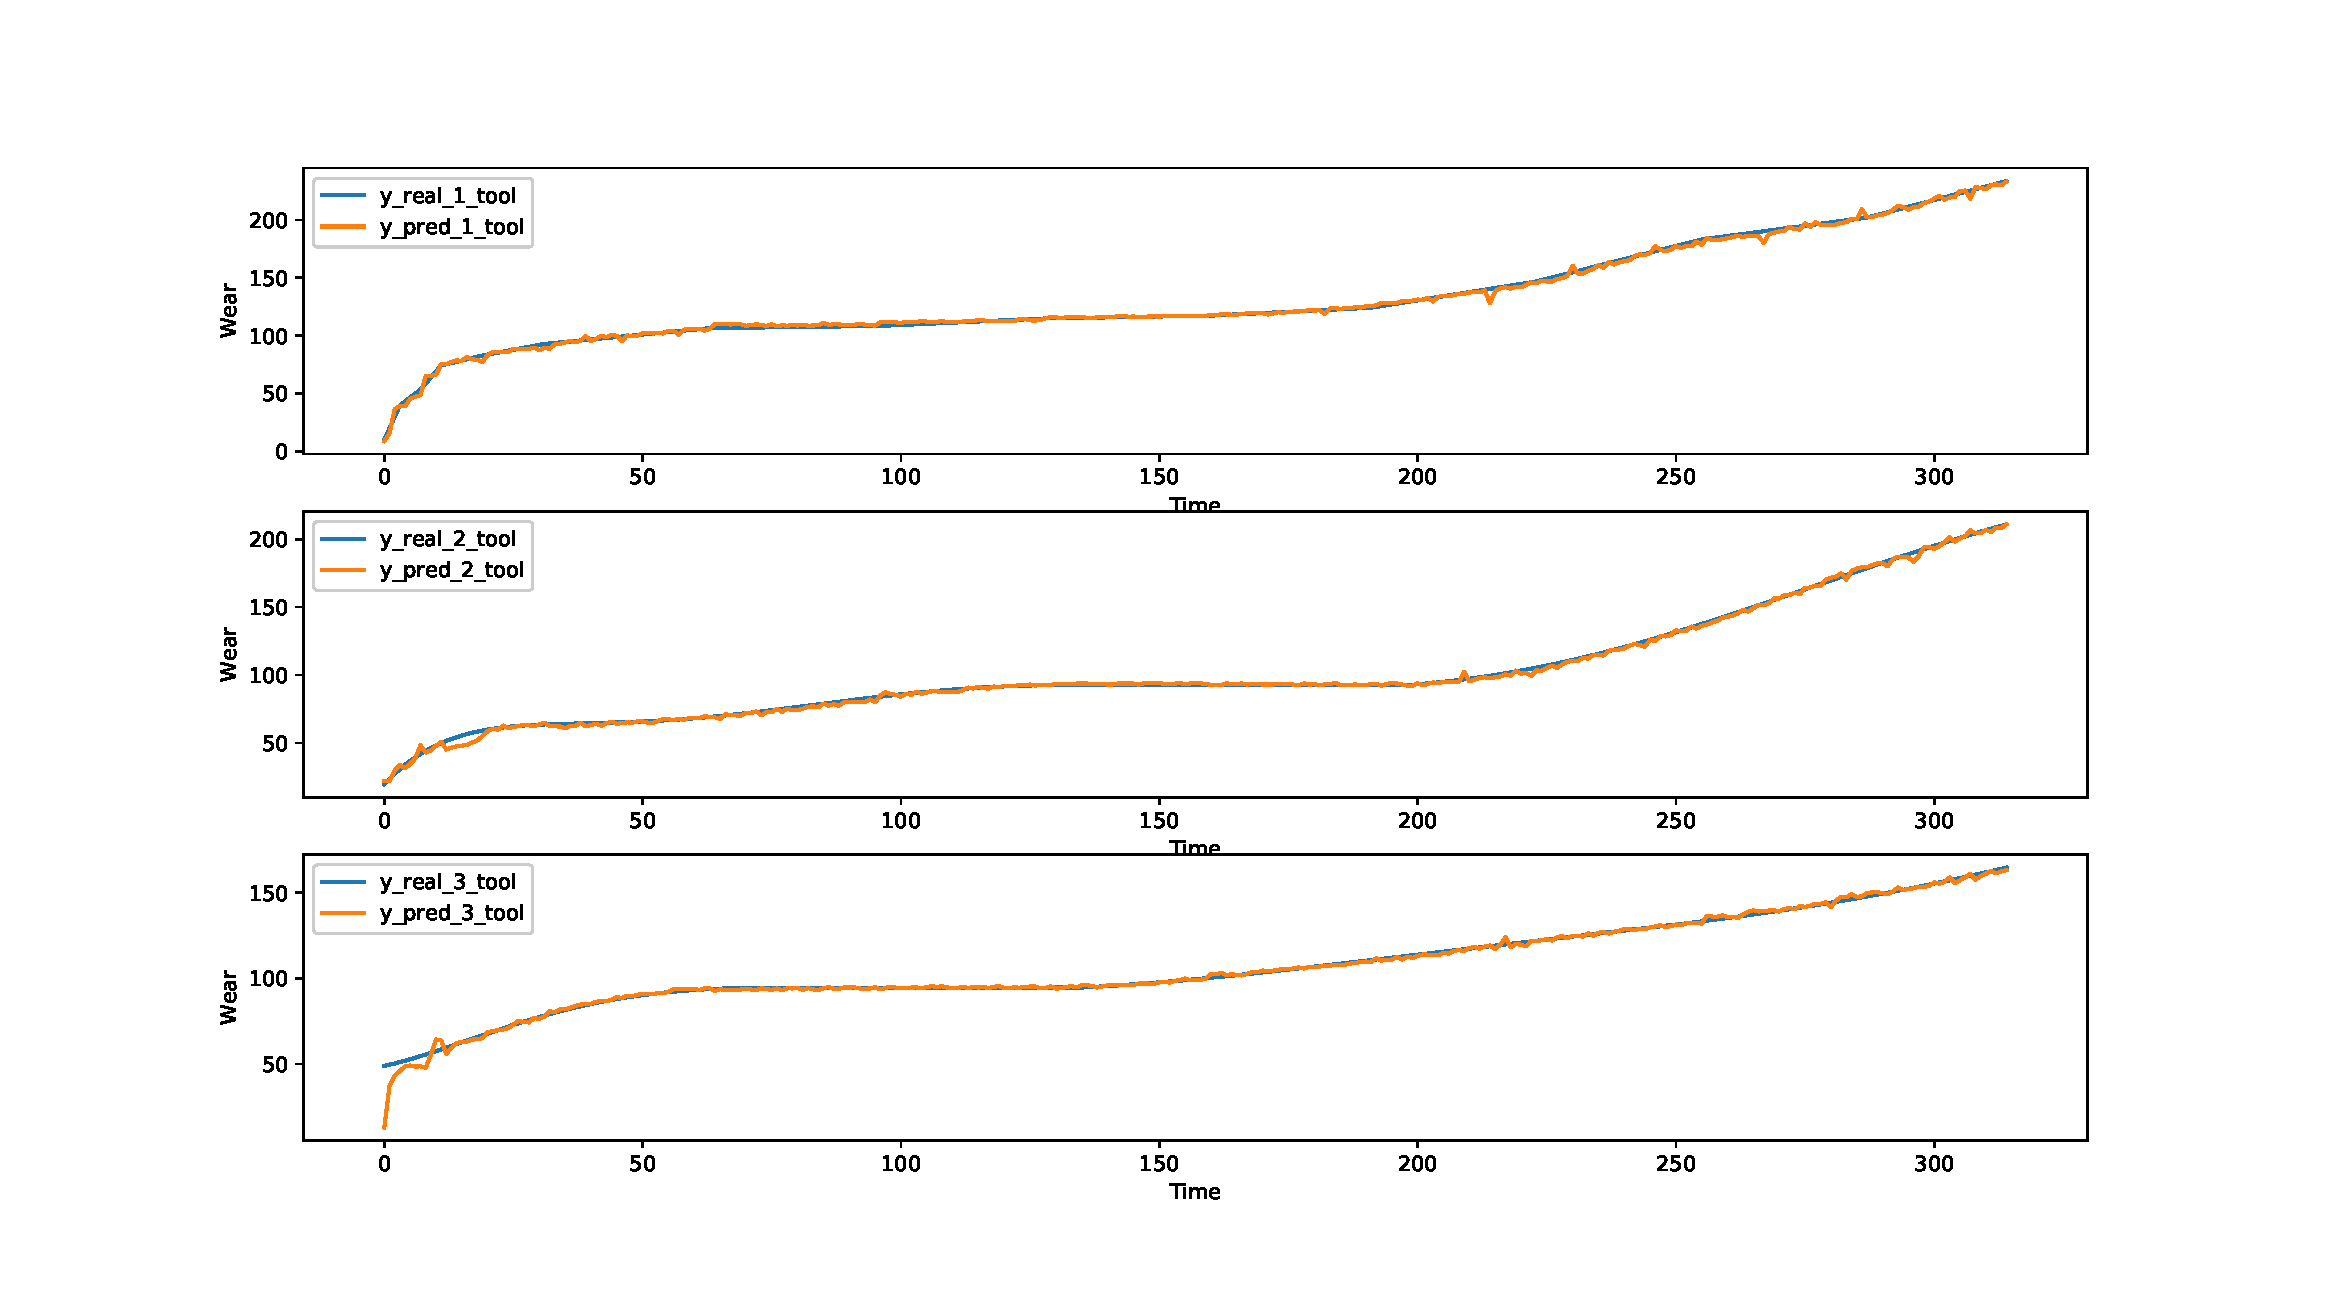
\includegraphics[height=0.9\textheight]{picture/y_tool}
		
	\end{frame}
	
	\begin{frame}{实验结果}
		\centering
		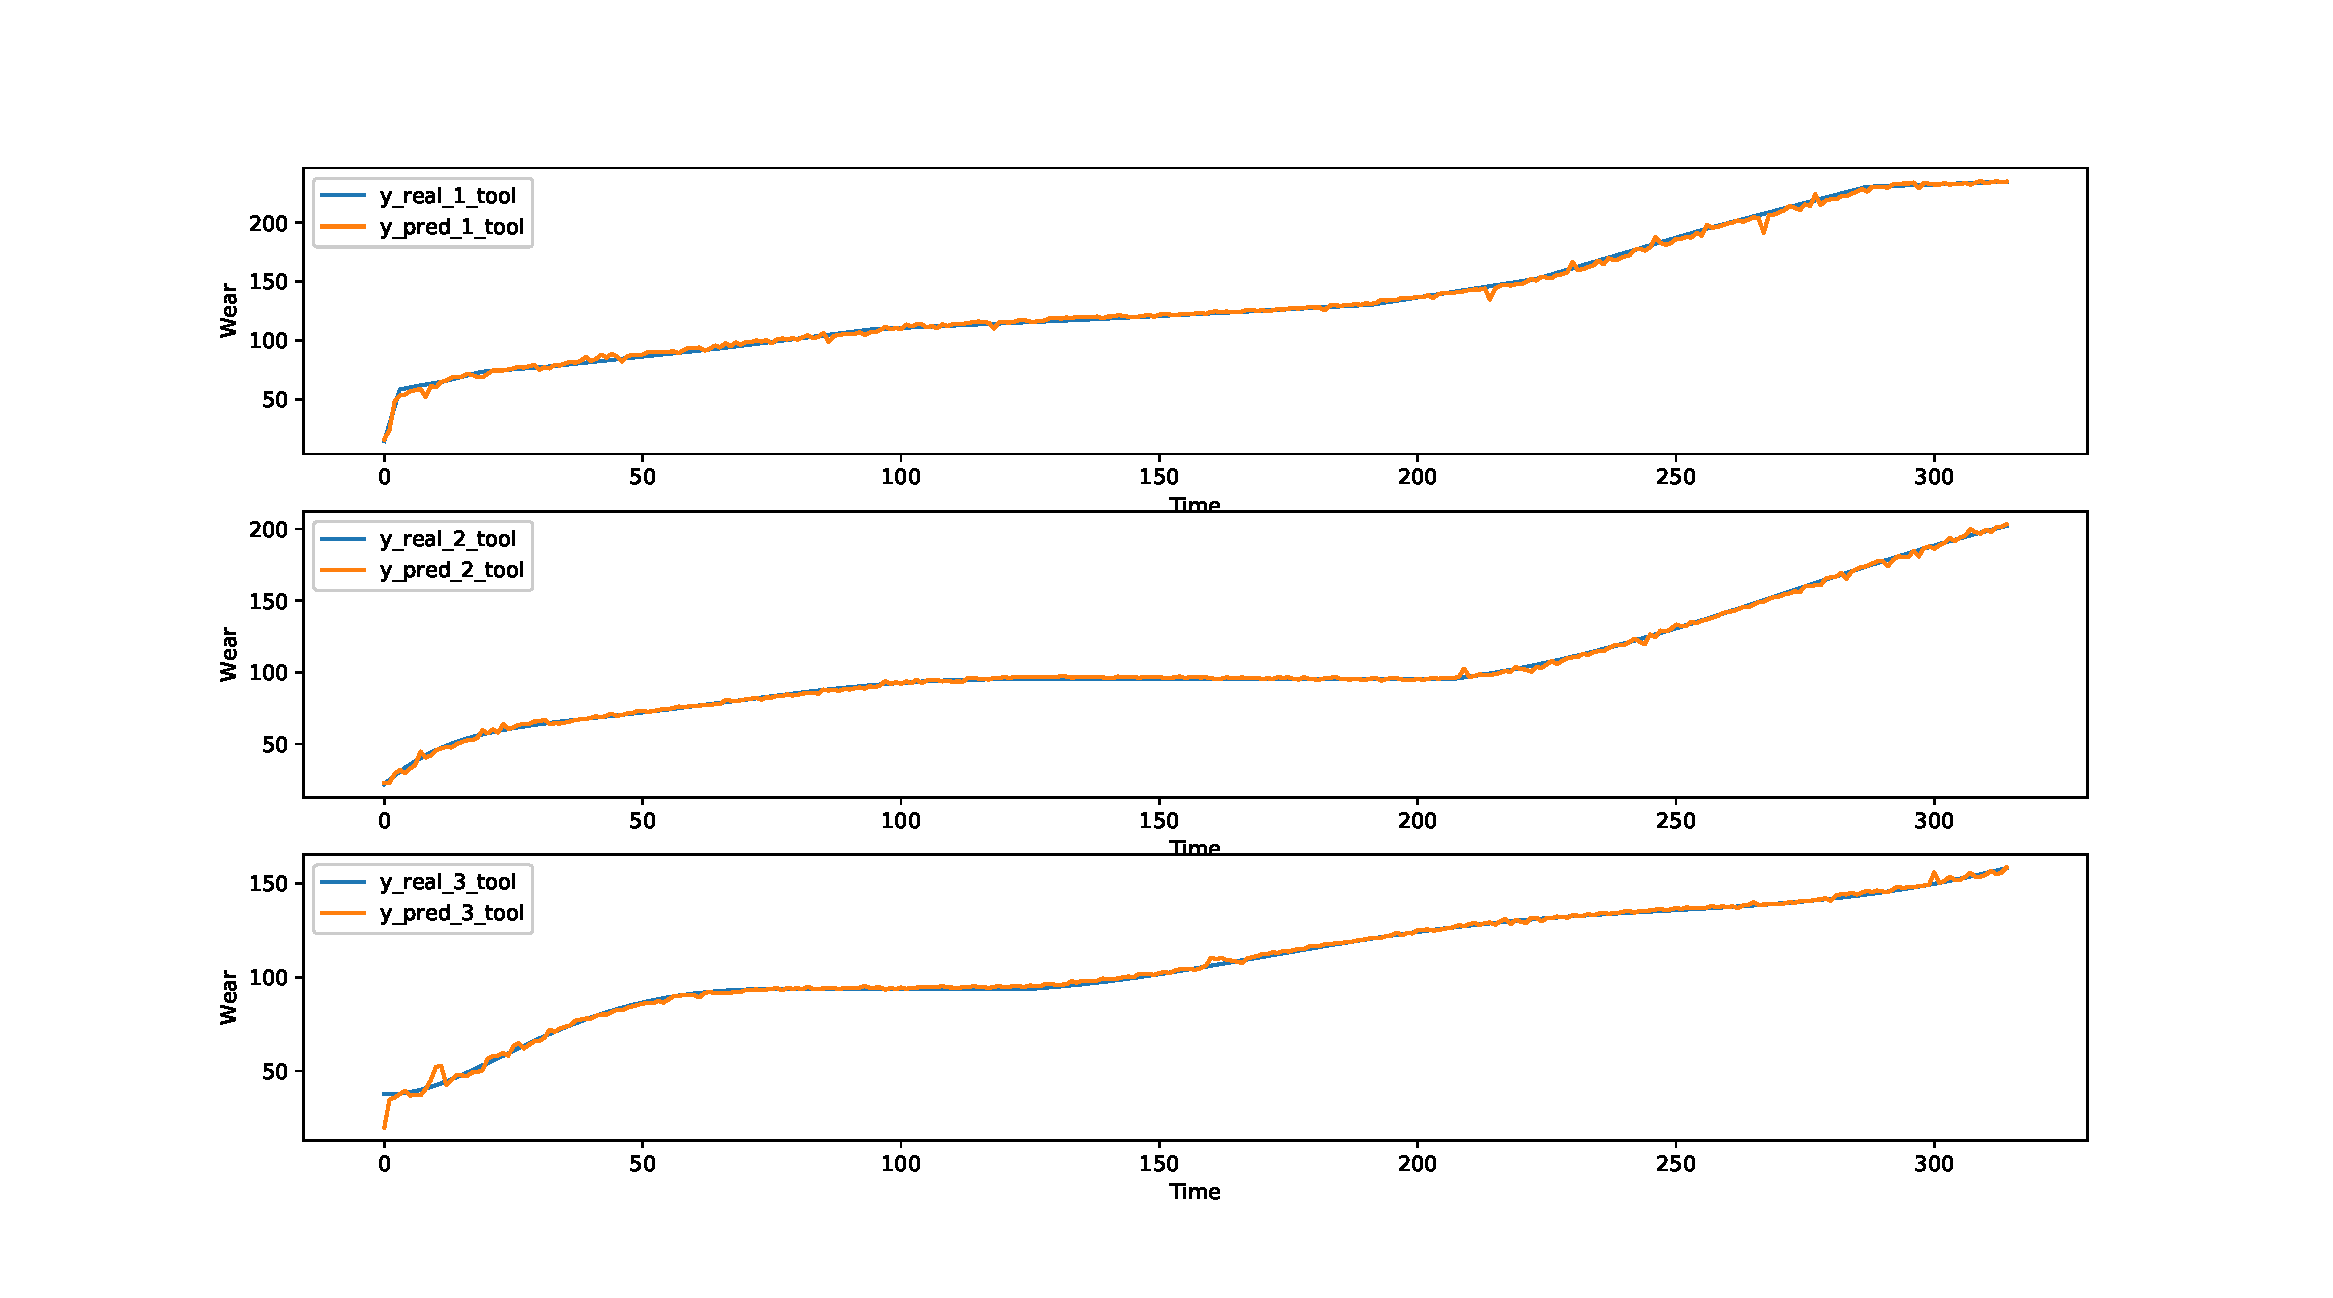
\includegraphics[height=0.9\textheight]{picture/z_tool}
		
	\end{frame}
	
	\begin{frame}{误差频率分布}
		
		
		\begin{columns}
			\begin{column}{0.33\textwidth}
				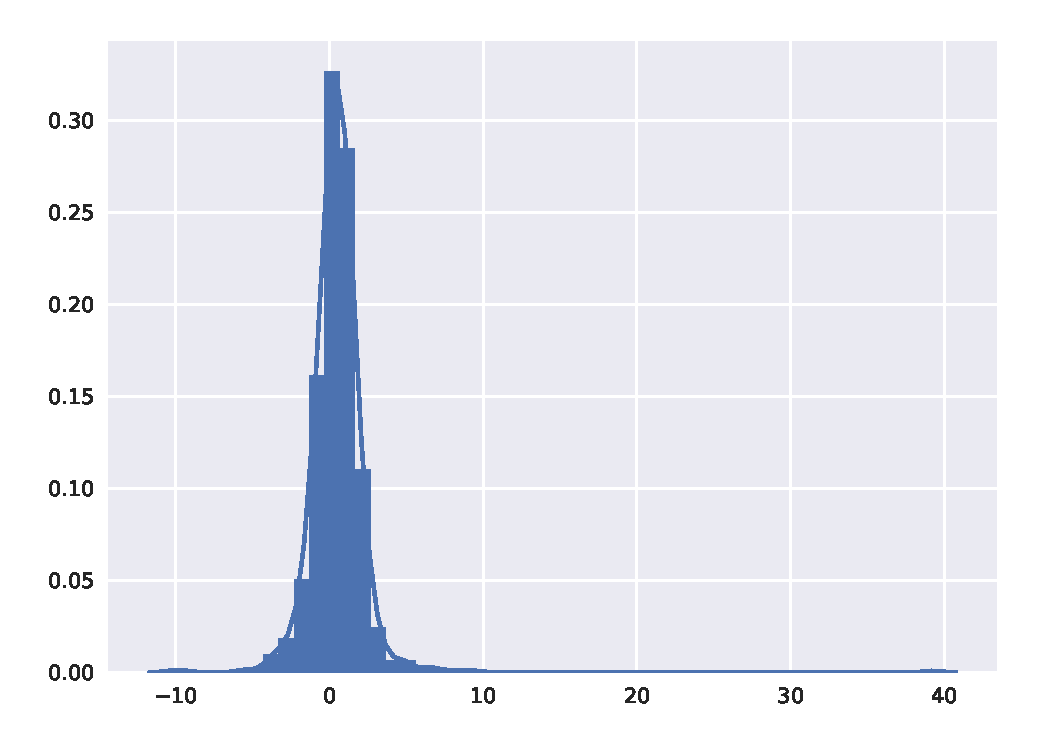
\includegraphics[width=\columnwidth]{picture/x_hist}
			\end{column}
			
			\begin{column}{0.33\textwidth}
				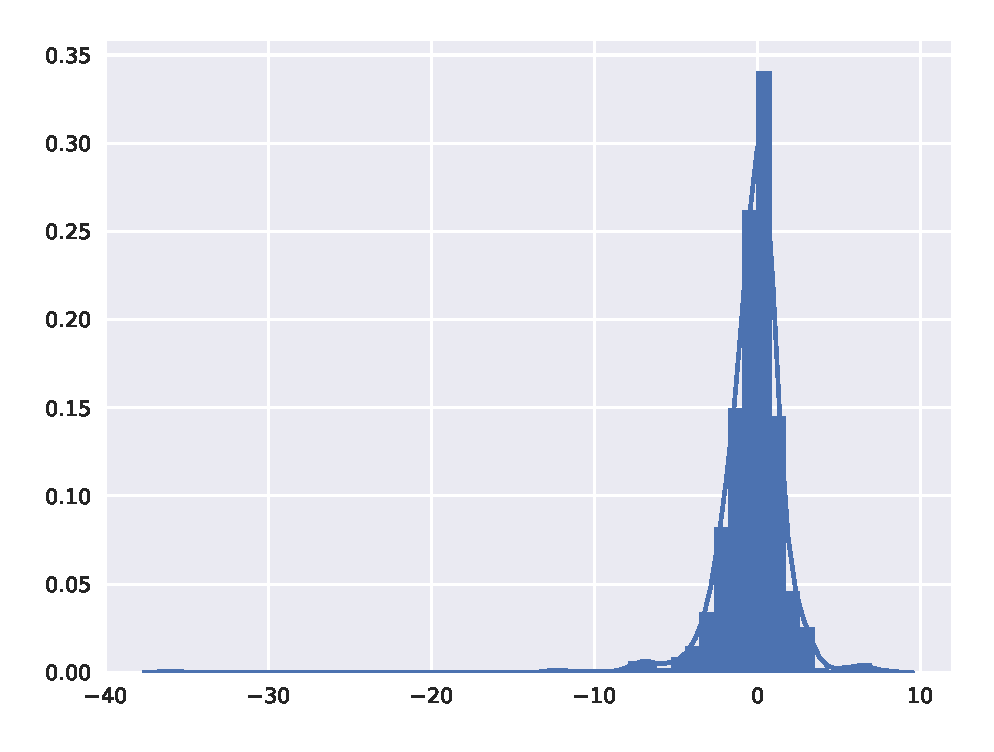
\includegraphics[width=\columnwidth]{picture/y_hist}
			\end{column}
			
			\begin{column}{0.33\textwidth}
				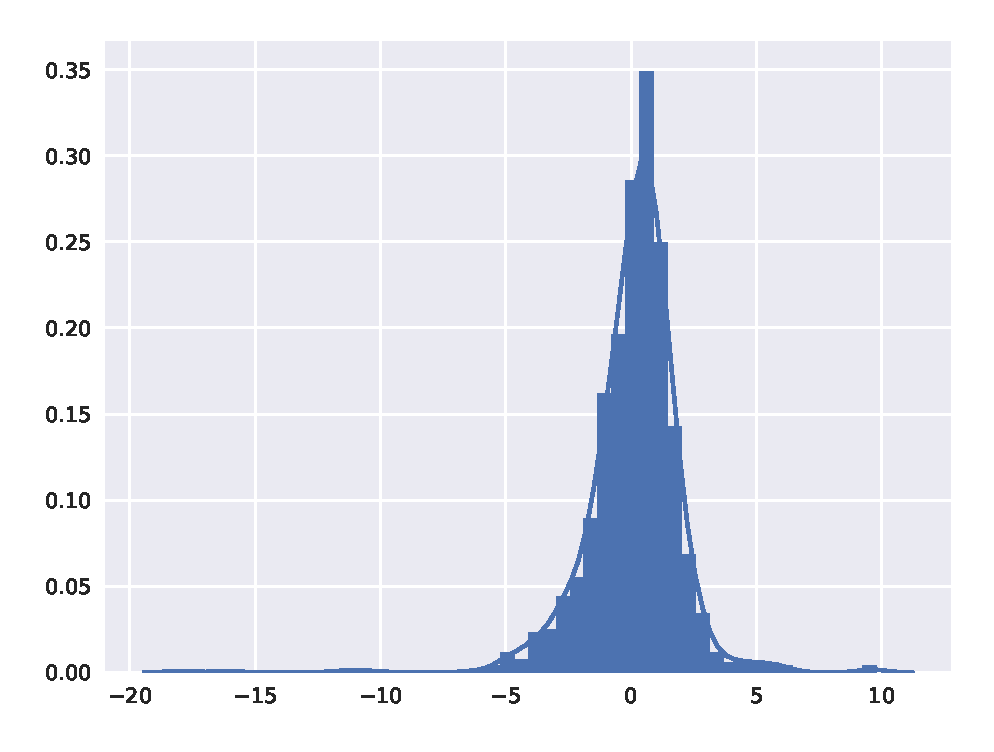
\includegraphics[width=\columnwidth]{picture/z_hist}
			\end{column}
			
		\end{columns}
	\end{frame}
	
	\begin{frame}{结论}
		\begin{enumerate}
			\item 残差剩余网络能够有效的预测刀具的磨损量(翻阅论文发现其也比基于阈值的方法更加稳健)
			\item 计算开销在基于CUDNN的计算环境下很小
		\end{enumerate}
		
		
	\end{frame}
	
	\begin{frame}{Reference}
		\scriptsize
		\bibliographystyle{apalike}
		\bibliography{Biblio}
	\end{frame}
\end{document}